\chapter{Présentation}

\section{Auteur}

\noindent
Corentin POUPRY, étudiant à l'ESIEE Paris en E1, promotion 2025.

\section{Thème}

\noindent
Murphy Law, un détective, doit faire la lumière sur l'enquête confiée.

\section{Résumé du scénario}

Vous vous attendiez à tomber sur un super jeu de science-fiction proposé par un étudiant talentueux. Cependant, la réalité est tout autre et vous vous retrouvez au bureau d'un curieux détective. Ce détective, bien décidé à vous aider à faire la lumière sur votre cas atypique, c'est Murphy Law, et c'est lui qu'on appelle quand tout va mal.

\section{Scénario détaillé}

Le Joueur (notons la majuscule) est un personnage à part entière de l'histoire, bien que l'utilisateur joue au travers de Murphy Law. Le Joueur apparaît au début de la narration complètement perdu et à la recherche du jeu de science-fiction promis par le talentueux étudiant dans son rapport. Murphy Law, détective, se demande par quel moyen Le Joueur a pu arriver dans son agence alors que, manifestement, il ne fait même pas partie du schéma narratif du jeu. Quelque chose cloche, quelque chose ne tourne pas rond.

Murphy Law décide de partir mener l'enquête en allant voir une source pouvant l'aider dans cette enquête. Avec Le Joueur, il monte dans sa voiture, cependant, la structure du jeu commence à se corrompre, à changer dangereusement sans raison, provoquant la stupéfaction chez les deux protagonistes. Murphy accélère pour semer les incohérences de narration. Alors qu'ils roulent vers leur contact à toute allure, Murphy commence à perdre le contrôle de la situation jusqu'à qu'un arbre apparaisse devant la voiture provoquant un accident.

Murphy Law et Le Joueur se réveille dans un grand escalier avec des dorures et un dôme imposant surmontant la pièce. Après l'irruption d'un majordome disant qu'on les cherche partout, Murphy et Le Joueur réalisent qu'ils passé dans l'univers d'un autre jeu de la promotion, prenant place à Buckingham Palace. Très vite, Murphy Law et Le Joueur sont accostés par les employés du palais, les prenant pour les détectives ayant été appelés par le palais pour retrouver un bijou de la reine manquant.

Cependant, en inspectant une cave du palais, Murphy Law et Le Joueur se retrouve propulsé dans un vaisseau spatial en pleine bataille stellaire. Ils comprennent assez vite qu'il ne leur reste pas beaucoup de temps avant que le vaisseau n'explose. Une fois la sortie trouvée, ils se retrouvent encore une fois propulsé dans le voiture de Murphy Law, ce dernier bien décidé à faire toute la lumière sur les récents évenements.

Murphy Law décide alors d'aller à l'ESIEE. Une fois arrivé là-bas et flairant que quelque chose se trame dans son dos, Murphy Law décide alors de se rendre là où tout a commencé : dans la salle où Le Joueur avait lancé le jeu. Murphy Law se retrouve alors confronté au Compilateur, qui essayait de manipuler le jeu pour que l'étudiant n'obtienne pas une note à la hauteur de sont travail. Murphy ressort gagnant de cette confrontation, ce qui lance le dialogue de fin de Planet Wars.

\textbf{Note :} En raison d'un manque de temps, je n'ai pas pu implémenté un système de dialogue assez complexe pour soutenir le scénario du jeu. Seul la partie technique est présente.

\section{Plan}

\begin{figure}[H]
  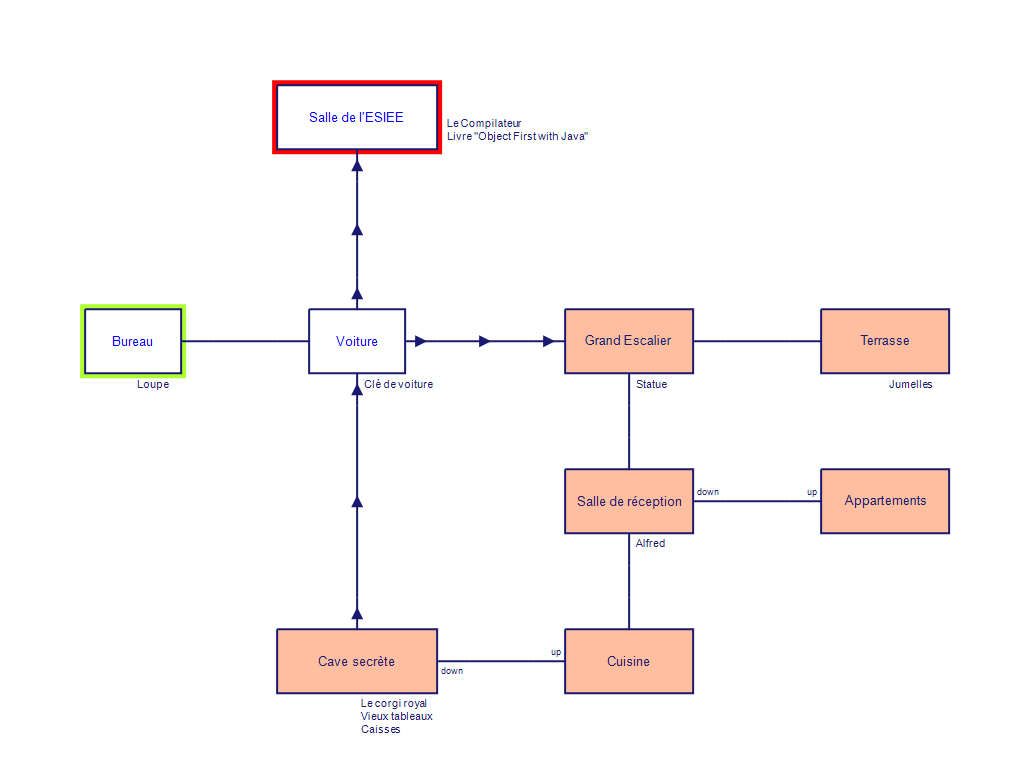
\includegraphics[width=\textwidth,height=\textheight,keepaspectratio]{./media/plan.png}
  \caption{Plan du jeu}
\end{figure}

\section{Détail des lieux, items, personnages}

\subsection{Lieux}

Seuls les lieux importants à l'avancement et à l'histoire du jeu sont listés ci-dessous.

\begin{description}[leftmargin=!,labelwidth=\widthof{\bfseries Palais de Buckingham}]
  \item [Bureau de Murphy] C'est le lieu où vous commencez votre aventure.
  \item [Voiture] La voiture vous permet de rejoindre certains lieux.
  \item [Palais de Buckingham] Là ou loge la reine et où Murphy Law ménera une courte enquête.
  \item [Salle de l'ESIEE] C'est dans cette salle de l'ESIEE que vous avez lancé ce jeu.
  \item [Vaisseau] C'est un vaisseau spatial inspiré de l'Enterprise de Star Trek.
\end{description}

\subsection{Personnages}

De la même façon, cette liste ne comprend que les personnages essentiels au scénario. Certains personnages non-joueurs ne sont pas listés ici.

\begin{description}[leftmargin=!,labelwidth=\widthof{\bfseries Le Compilateur}]
  \item [Murphy Law] Le détective et aussi le personnage que vous incarnez. Son rôle est de mener l'enquête pour comprendre par quelles circonstances Le Joueur s'est retrouvé ici.
  \item [Le Narrateur] La voix que vous entendez quand vous jouez. Le Narrateur permet de décrire les scènes et situations sans sortir de la narration. 
  \item [Le Compilateur] Le compilateur Java est le grand méchant de l'histoire. Son rôle, manipuler la structure du jeu pour que l'étudiant n'ait pas une note à la hauteur de son travail.
\end{description}

\section{Commentaires}

Murphy Law est une création originale de \href{http://scp-wiki.wikidot.com/murphy-law-hub}{la Fondation SCP}. Le personnage, les oeuvres associées et ce jeu sont tous proposés sous licence \emph{Creative Commons Attribution-ShareAlike 3.0}

\subsection{Important}

Pensez à compiler à la main le fichier \code{ZuulController} car BlueJ ne le fait pas.
